\section*{Project Description}

\todo{GPG: Proposals should identify a computer and information
  science and engineering grand challenge and an agenda to tackle such
  a challenge.}

\todo{GPG: proposals should explain why existing CISE core programs
  for Small and Medium size projects
  (\$600,000 over three years and \$1,200,000 over four years,
  respectively) are inadequate to address the grand challenge. A
  strong rationale must be provided that explains why a budget of this
  magnitude is required to carry out the proposed work.}

\todo{GPG: The proposal must explicitly identify the participating
  CISE core programs it covers and make the case for why the challenge
  is within the scope of one or more of these participating core
  programs.}

\todo{Webinar: Proposals must be clear about why this kind of scale is
  required for the research to succeed.}

Testing plays a vital role in modern software development,
contributing crucially to robustness and overall quality---as well as
to overall development costs.
%
It comes in many styles---unit testing, integration testing,
performance testing, stress testing, accessibility testing,
etc.---supported by many sorts of tools, with yet more advanced tools
and techniques continually being developed, studied, and applied.

One such technique, {\em property-based testing} (PBT), has been
enthusiastically taken up by the functional programming research
community since its introduction in the Haskell QuickCheck
library~\cite{ClaessenHughes00}, and is beginning to make
serious inroads beyond academia.
%
PBT is sometimes glossed as ``formal specification without formal
verification'': a developer characterizes the desired behavior of
some piece of code at a high level in the form of executable {\em
  properties}, which are simply Boolean-valued functions. The code is
then validated against these properties by running it over and over
with a large number of automatically generated test cases.
%
PBT tools thus give programmers an efficient way of testing their
code's behavior with a comprehensiveness that is often not
possible with alternative testing methods.

PBT's combination of rich, high-level specifications with easy, mostly
automatic validation has shown itself effective at identifying subtle
bugs in an impressive variety of settings, including telecommunications
software~\cite{arts2006testing}, replicated
file~\cite{hughes2014mysteries} and key-value
stores~\cite{Bornholt2021}, automotive software~\cite{arts2015testing}, and a range
of other real-world systems~\cite{hughes2016experiences}. With support
now available in pretty much every major programming language, PBT has
begun to make significant inroads in the broader software
industry. For example, the developers of the Hypothesis library for
Python estimate that it is used by around half a million
developers~\cite{ZacPersonalCommunication}.

\newcommand{\participant}[1]{{P#1}}
% \newcommand{\participant}[1]{{\bf P#1}}

Given all this momentum, one might wonder if the research community has
already
addressed all of the challenges that could limit PBT's adoption
in the broader software industry.  But it
seems the answer is no.
In an ongoing need-finding study with users of OCaml's QuickCheck testing tool
at Jane Street Capital, we found
consistent enthusiasm for PBT---participants called it it
``obviously valuable'' (Participant \participant{1}),
built their own libraries for it when standard ones were not available
(\participant{8},
\participant{21}), and suggested that ``everyone'' at the company should use it
(\participant{20})---but participants also described {\em usability} issues
that demand advances in technical foundations and
tool design.

Addressing usability challenges in PBT requires insights from both the
programming languages (PL) and
human-computer interaction (HCI) communities.  Chasins et
al.~\cite{chasins_pl_2021} argue that a research methodology
combining PL and HCI hits a ``sweet spot'' where need-finding techniques identify
current pain points and motivate concrete tools that help programmers write
safe, correct programs. We wholeheartedly agree.
Indeed, the team behind this proposal is uniquely positioned to advance the
state of the art in PL and HCI: PI Head recently co-founded
a new HCI group at the University of Pennsylvania and specializes in interactive
programming environments, while PI Pierce has
published widely on PL topics including PBT.

We propose here a comprehensive, interdisciplinary research program on
\emph{usable
property-based testing}, bringing the combined power of PL and HCI to bear to
accelerate PBT's transition into practice.
\begin{itemize}[noitemsep]
% \begin{enumerate*}
\item We will establish a \emph{foundation} for HCI-informed research on PBT,
starting from our ongoing need-finding study. We will confirm
this study's findings and more deeply explore usability of PBT via
two survey studies and an observation study
of PBT users {\em in situ} (\sectionref{sec:foundation}).
  \item We will empower developers to \emph{specify} properties with
  new tools for checking temporal properties over internal program states and
for model-based testing of modularized code (\sectionref{sec:spec}).
  \item We will help developers efficiently define and tune random input
\emph{generators} with novel techniques for generating precondition-satisfying
values, for test input mutation, and for example-based generator
tuning, all building
  on a novel ``reflective'' approach to generation (\sectionref{sec:gen}).
  \item We will support developers in rapidly \emph{validating} testing
  effectiveness with novel interactive tools that help
locate causes of test failures and understand how to improve the
distribution of randomly generated
data to be more representative and comprehensive
(\sectionref{sec:val}).
  \item We will develop materials for PBT \emph{education}
  including an undergraduate computer science curriculum centered around PBT, a
  tool to help students author properties, and a comprehensive review of PBT
  practice to help students and developers identify situations where
  PBT is likely to be most useful (\sectionref{sec:ed}).
% \end{enumerate*}
\end{itemize}
%
Success in these efforts will require complementary tools from PL
and HCI research. HCI approaches will be used to concretely define developers' needs,
design the user interface to tools, and evaluate their success. PL approaches
will be used to develop powerful domain-specific languages and type-based automation
to improve the PBT process, as well as to formally validate these
tools. The proposal concludes with a concrete outline of our work plan
(\sectionref{sec:plan-of-work}), a discussion of the broader impacts of the
proposed work (\sectionref{sec:broader-impacts}), and a summary of our
prior NSF-supported work.

\subsectionstar{Orientation: Property-Based Testing}
%
Popularized by Haskell's QuickCheck library~\cite{hughes2007quickcheck},
PBT is a form of testing where
executable functions act as partial
specifications of a component under test. For example, a user might
write the following property for an \lstinline{insert}
function for a Binary Search Tree, taking an arbitrary tree \texttt{t}
and an integer
\texttt{x} to insert into that tree as parameters. If the original tree
is a BST, then it should remain
a BST after the insertion of \texttt{x}:
\begin{lstlisting}
  prop_insert_correct x t  =  (is_bst t ==> is_bst (insert x t))
\end{lstlisting}
In general, a property is a function that
accepts a generated
test as input and evaluates to \lstinline{True} if the test passes, and
\lstinline{False} otherwise.  This one, ``\verb|prop_insert_correct|'',
checks that an insert operation on a binary search tree preserves the
binary ordering of the tree.
Given a property, the PBT tool generates a
large number of inputs and
checks that the property yields \lstinline{True} for each one; any input
that causes the property to fail is reported as a {\em counterexample}.

This proposal focuses on {\em random}
generation~\cite{hamlet1994random}, the dominant approach in PBT,
though many of our tools would
also be applicable to alternatives like enumerative test-case
generation~\cite{DBLP:conf/haskell/RuncimanNL08, leancheck}.
The surprising effectiveness of random generation can be attributed to the
``combinatorial'' nature of larger test cases---the fact that bugs can often be
exposed with test inputs that embody a specific combination of features,
independent of whatever other features may be present. For example,
a bug might be triggered by a particular sequence of API calls in a
particular order,
regardless of whether these are
interleaved with other API calls. As a result, testing with large random
inputs often exposes issues much faster than exhaustively enumerating
small inputs.  Techniques like swarm testing~\cite{groce2012swarm} can
further amplify this effect.

To apply PBT, the developer first defines one or more properties that
should be true of the program under test. Then, they write {\em random
  input generators} for the values that the properties take as input
(often these can be automatically generated). Next they check the
properties with generated inputs, using test drivers provided by their
PBT tools. And finally, if counterexamples are discovered, they make
sense of them and determine the source of the bug.  Each of these
steps presents opportunities to improve the user experience of PBT, as
we describe in the next section.

\smallskip

Why go to the trouble of PBT, rather than the more straightforward
example-based testing that is standard across the software industry?
First and foremost because a component can be tested be much more
thoroughly with a property and many automatically generated examples
than with a small number of examples written out by hand.
% \proposecut{As mentioned
% previously, PBT has an impressive track-record uncovering bugs that other
% approaches had failed to
% find~\cite{arts2006testing,hughes2014mysteries,
% Bornholt2021,arts2015testing,hughes2016experiences}.}
But
PBT is more than just thorough---it is also more general than example-based
testing. Wrenn et al.~\cite{wrenn2021using} point out that example-based testing
of programs whose correctness conditions are {\em relational} (e.g.,
topologically sorting a graph, which might
produce any of a number of correct results) is impossible to do
faithfully; a property-based specification is a better choice in
such cases.
PBT is also
an obvious choice if
the developer already has some semi-formal
specification in mind, for example if they are implementing behavior from an RFC or
other design document, because it provides a clear connection between the
specified behavior and the implementation.
Finally, the
properties required for PBT can also serve as documentation:
participants in our foundational study (\participant{5}, \participant{21})
talked at length about properties being an ideal way to communicate what a
program is supposed to do.

With all these advantages, it seems clear that PBT belongs on every
software developer's testing toolbelt.  But PBT raises some challenges
as well, as we shall see next.

\subsectionstar{Motivations from a Formative Study of PBT in
Industry\label{sec:motivation}\pagebudget{2}}
%
The work proposed here is motivated by findings from the
need-finding study we are conducting at Jane Street. The purpose of this
study is to understand how the research community can make PBT more
usable. The study data consists of thirty semistructured interviews
with developers who use PBT and maintainers of PBT tools.

Jane Street is
an attractive setting for this study for several reasons.  First and most
importantly, PBT is
already well established at Jane Street, so there is a large
population of people with well-informed opinions on its benefits and
challenges. Additionally, Jane Street famously builds nearly all of its
software in OCaml, a mostly functional programming language for which
there is a well-engineered PBT tool. This unified
ecosystem ensures that developers have access to mature PBT tools,
experience using them in collaborative settings,
and awareness of language-level abstractions necessary
for advanced usage.

As of December 2022, the full complement of thirty interviews has been
completed at Jane Street, and a preliminary round of qualitative
analysis is underway; full-scale analysis will begin in 2023.
Findings from the study will be disseminated in a paper submitted to a
top-tier software engineering conference.  We also carried out a
smaller pilot study among Hypothesis users to prepare for the
full-scale one at Jane Street; this study was presented at the
2022 HATRA workshop~\cite{goldstein_problems_2022}.

\subsectionstar{Framework: Challenges Using PBT} The final result of
the ongoing study will be a fine-grained, qualitative description of how
Jane Street developers use PBT, what they need from it, and how the
research community can
help improve PBT tools. While full analysis of the data remains
to be done, a number themes are already clear. These form the backbone
of the present proposal.

\newcommand{\proptheme}[1]{{\color{nord-orange} \em #1}}
\newcommand{\gentheme}[1]{{\color{nord-green} \em #1}}
\newcommand{\evaltheme}[1]{{\color{nord-purple} \em #1}}
\newcommand{\edutheme}[1]{{\color{nord-frost4} \em #1}}
A first set of
themes revolves around \proptheme{\normalfont \bf specifications} (i.e.,
properties).
% and the kinds of programs in which they choose to test them.
Since
PBT is often described as a lightweight formal method, one
might imagine that a common challenge would be coming up with the
specifications of desired program behavior. Indeed, in our earlier pilot
study~\cite{goldstein_problems_2022}, some users indicated just that.
By contrast, Jane Street developers, on the whole, reported
little difficulty finding
properties. Rather, most developers applied PBT in
\proptheme{High-Leverage Scenarios} where properties were already
available or straightforward to invent. In participant
9~(\participant{9})'s words, PBT is particularly easy to apply when one
has ``a really good abstraction with a complicated implementation.''
Several developers (\participant{3}, \participant{15},
\participant{20}, \participant{22}), when asked to speculate, guessed
that 80--100\% of Jane Street
developers write programs like this, where properties are easy to find and
PBT is relatively easy to apply. This suggests that an effective way to
improve education and documentation for PBT would be to highlight
real-world applications that are a natural fit.

We also heard \proptheme{Opportunities for Better
Leverage} of specifications, where PBT is not easy {\em yet}, but
could be with a little more research effort. For example, developers in
both studies (Pilot-\participant{4--6}) and Jane Street (\participant{7}) complained
that PBT was difficult when code was poorly abstracted.  Further,
more than three
quarters of study participants had used a particular approach to PBT commonly
called \proptheme{Model-Based Testing}.  \participant{3}, an author of PBT tools
at Jane Street, considered better automation and tooling around model-based
testing to be one of the most significant ways improve PBT usability.

A different set of themes concerned the \gentheme{\normalfont \bf generation} of
random inputs for PBT. Developers spoke
highly of the \gentheme{Derived Generators} that can be automatically
inferred from
the OCaml type system (\participant{5} called OCaml's tools for this
``[expletive] amazing'' and \participant{30} called them a ``game changer'').
These generators are already quite good, but they could be better: participants
identified deficiencies both small (e.g., API quirks) and large (e.g.,
derived generators
cannot enforce semantic preconditions).

When derived generators
failed, participants fell back to \gentheme{Bespoke Generators}, which
are far more flexible but proportionally more time-consuming to
build. For example, \participant{20} successfully used a bespoke
generator for XML documents to find significant bugs in their code,
but reported spending ``at least a day'' writing it.
Improving the abstractions available for authoring bespoke generators would
greatly improve the usability of PBT.
%
When a generated input turns out to be a {\em counterexample} that triggers
a property violation, the developer will need to inspect that
counterexample to find
and fix the root problem. Developers often implemented code for
\gentheme{Shrinking} counterexamples to discover smaller,
simpler inputs that trigger the same bug.  \participant{8}
and \participant{21}, who each implemented their own PBT libraries, both
incorporated shrinkers as key components of their libraries. But
shrinkers need to be customized to particular kinds of data to be most
effective, and they can be time-consuming to build; several
developers
(\participant{16}, \participant{20} \participant{21}, \participant{30})
described shrinker implementation as an opaque and difficult process.
Ideally, developers would have tools that make the process of implementing
shrinkers fast and simple.

A further set of themes concerned
\evaltheme{\normalfont \bf validation}---the processes developers use
for \evaltheme{Evaluating the
Effectiveness} of their tests. Many
desired
better ways to evaluate their generators and properties, including
better feedback on code coverage (\participant{9} and \participant{25}),
incorporation of mutation
testing~\cite{papadakis_mutation_2018}, and help understanding the
distribution of randomly generated
inputs (\participant{10}, \participant{16}, \participant{16}). Problematically,
while many developers admitted they would benefit from better tools for
evaluating their tests, many seemed to
\evaltheme{Implicitly Trust the Infrastructure} that they did use. \participant{14} actually shipped broken code to production because
they did not realize their generator had missed important input
examples.

Finally, both of our studies reveal a need for progress
in PBT
\edutheme{\normalfont \bf
education}. Developers need to be informed about the \edutheme{High-Leverage
Scenarios} in which PBT should be employed, as discussed above.
In the pilot study, we found that developers with less experience with PBT
sometimes struggled to \edutheme{Imagine
Properties} or to understand what properties to test (Pilot-\participant{1},
Pilot-\participant{3},
Pilot-\participant{4}, Pilot-\participant{5}). Developers in both studies
(Pilot-\participant{1}, Pilot-\participant{4}, \participant{3}, and
\participant{11}) reported a dearth of \edutheme{Documentation and Examples} for
learning about PBT.

We discuss plans for work that addresses \proptheme{specification
  themes} in \sectionref{sec:spec}, \gentheme{generation themes} in
\sectionref{sec:gen},
  \evaltheme{validation themes} in \sectionref{sec:val}, and \edutheme{education
  themes} in \sectionref{sec:ed}.  To support all of this work,
\sectionref{sec:foundation} describes plans for a further round of
studies to deepen our understanding of PBT needs and opportunities
across a wide range of industrial settings.

% \iflater
% \amh{Let's foreshadow other findings that
% we will publish that are outside of the scope of this proposal, but which might
% be motivating to other researchers, including: developers could benefit from
% additional automated support for deriving generators from types, effectiveness
% budget (i.e., deciding how much time to spend on running PBT tests versus fuzz
% tests), integration with unit testing frameworks, and exploring the use of
% properties as a source of documentation.}
% \bcp{Not sure where is the right place for this discussion (or if
%   there will be space)...}
% \fi

\SECTION{Foundation}{Understanding Needs and Opportunities%
\pagebudget{1}}{sec:foundation}

% \amh{This section is around double its page budget. One reason is that I am
% probably being too heavy-handed in trying to justify the methodological choices.
% Help me figure out what to prune!}\bcp{Did some pruning! :-)}

The final results from the in-progress user study will paint a clear
picture of the benefits and challenges of PBT in the specific context
of Jane Street and other organizations with similar characteristics.  But to
fully understand the potential impact of PBT across the software
industry---and the factors that may limit its adoption---we need to
cast a wider net.
%
In this section, we describe three planned studies, drawing on mixed
methods in the service of producing a comprehensive and actionable
agenda for research in this project and beyond: two
written surveys, one to assess the generality of these needs and obstacles
and one to identify potential for adoption of PBT tools
(\sectionref{sec:survey}), and an observation study to understand
particular tasks involved in PBT to guide the design of new algorithms
and interactive tools (\sectionref{sec:observations}).

\SUBSECTION{Generalizing the Jane Street Findings}{sec:survey}{1}{2}{Andrew}
%
The Jane Street study has already revealed a number of
opportunities to improve tools for property-based testing. To identify
others and to better understand which of these opportunities are most
important for the research community to explore, we will conduct two
surveys with broader samples of developers. These surveys aim to
(1) determine which obstacles observed in the interview study
represent widely experienced pain points and
(2) characterize the potential benefits of better tools to the
software industry as a whole.

\TASK{Validation survey}{1}{2}{Who???} The main survey we will conduct
checks that
the things we are learning from Jane Street generalize to other settings.
We will
ask developers which of the issues are
ones they have also encountered, what the severity of those issues is
in their experience, and about
other issues they have encountered.
To provide
clear usage scenarios to guide research, respondents will
be asked to write brief anecdotes elaborating on the
most severe issues they remember.  Other questions will assess how
heavily respondants depend on specific features of their PBT tools
that may be enabled by their
ambient programming environment and language (e.g., whether their
language supports Haskell-like typeclasses or OCaml-style
metaprogramming, both of which have been used to good effect by
PBT tools in those languages).

Respondents will
be recruited broadly, from three sources: (1)
users of the Python Hypothesis framework; (2) Jane Street, aiming for
a broader set of developers in the interview study; and (3)
word of mouth and via announcements on the PIs' Twitter and Mastodon
accounts, various mailing lists, and discussion boards for developer
conferences---e.g., ``Yow!'', where PI Pierce spoke this
year~\cite{Pierce:Yow22}.
% Types and types-announce mailing lists. They are mailing
% lists for the types programming. We will distribute announcements among
% attendees of conferences like ICFP or ``Yow!'' whom have
% a cumulative thousands of programmers with functional
% programming experience.

\TASK{Impact survey}{1}{2}{who???} A more speculative survey we hope to
conduct\todo{Promise it!}
will investigate
how broadly PBT may {\em eventually} be able to reach.  To get a sense
of this, we will
survey ``proximal'' users of PBT---developers who do not use PBT
currently, but who might find it particularly
useful.  Particular attention will be given to those whose work requires the
writing of validation code and public APIs with some definition of types. We
will recruit a broad sample of participants across development contexts
(professional, open source, educational) by working with our industry contacts
and by recruiting over social media. Admittedly, this survey seems more
difficult to ``get right,'' and the design will evolve over time as we gain a
better understanding of the situations where PBT is most effective
(see \sectionref{sec:whento}), but if done right this could provide invaluable
feedback to PBT researchers about how far their work could reach.

\SUBSECTION{Observing PBT in Practice}{sec:observations}{2}{3}{Andrew}
%
Anecdotes related in interviews do not, in and of
themselves, generally provide enough information to inform the design of
effective tools---they beg questions like: (1) How much time
are participants willing to devote to
a task like creating a property or tuning a generator when in the
middle of a programming task? (2) How much space is available on a developer's
screen (amidst other tools like code editors and terminals) for
new
tools? and (3) What are developers' current strategies for solving the
problems they describe---e.g., what representations of generated data
currently seem most helpful
for programmers trying to understand the distributions of data generated by a
generator? As a basis for designing tools with a substantial novel interface
component (see \sectionref{sec:val}), we will observe a modest number
of developers (perhaps 2--10 observation sessions)
undertaking PBT tasks similar to the ones we
aim to support. These observations will allow us to evolve
singular anecdotes from the interviews into a more comprehensive picture of
the kinds of designs that will help programmers.

\SECTION{Specification}{Widening the On-Ramp\pagebudget{2}}{sec:spec}
%
% To widen the on-ramp to using PBT, developers need help envisioning and
% writing \proptheme{specifications}. Developers first need to know when they
% should write properties to test their software. We describe our approach towards
% helping them do so in among our educational agenda~\sectionref{sec:whento}. In
% this section, we describe specific tooling that, once a developer has a property
% in mind, helps them implement it. We envision how tools can help developers
% poorly abstracted code (\sectionref{sec:outpurprop}) and test systems using
% model-based specifications (\sectionref{sec:automating}).
% \hg{I sort of liked what was here before... See comment}
%
A notable finding of the Jane Street study has been that widening the
on-ramp to PBT requires making developers aware of high-leverage
use-cases for PBT. Our plans to teach developers about high-leverage
scenarios are described below in \sectionref{sec:whento}; here,
we discuss research opportunities that can help expand this space.
Specifically, we describe plans to improve PBT's applicability to
poorly abstracted code (\sectionref{sec:outpurprop}) and
tools that will automate automatically in the specific high-leverage
scenario of model-based testing (\sectionref{sec:automating}).
The findings of the Jane Street study suggest that progress in these
two areas will significantly widen the on-ramp to PBT.

\SUBSECTION{Properties Over Logs}{sec:outpurprop}{2}{3}{Benjamin}
% With current PBT tools, properties can only be expressed over single modules.
% This causes problems when code is organized with functionality crossing module
% boundaries.
A common pain point for developers in our formative research
was that code may not be organized in a way that is conducive to property-based
testing. As a unit testing technology, PBT requires ``units'' of software to
test with clear boundaries. As such, PBT cannot easily apply to programs with
poorly encapsulated global state, or software with leaky or complex abstraction
boundaries.

Could there be a class of PBT tools that supports checking properties of
software in cases where important functionality falls across module boundaries?
We will explore how a PBT tool can support the definition of properties over
cross-module event logs. To demonstrate the potential of such a tool, consider
the case of a developer we interviewed, \participant{7}. P7 was testing
a system, which we call ``\lstinline{Inner},'' exemplifying this messy
abstraction
boundary. It was difficult to test \lstinline{Inner} because
its most interesting behavior arose only when interacting with its calling
component (which we call ``\lstinline{Outer}'').
\lstinline{Outer} took in simple inputs, and used these inputs to construct
complex inputs to \lstinline{Inner}. \lstinline{Inner} could not be tested with
realistic inputs without the complex apparatus of \lstinline{Outer} that
produced those inputs. The developer named this as a circumstance where a
PBT is difficult to apply, because the abstraction boundary between the
components is too fuzzy.

We will develop a tool that allow developers to express properties that reach
into the state of multiple interacting software components. Take again the
example of \lstinline{Inner}. A solution to P7's problem could be to drive the
test through \lstinline{Outer}, and in doing so implicitly test
\lstinline{Inner}, monitoring runtime values within \lstinline{Inner}. Assuming
\lstinline{Inner} is a routine that processes a stream of messages with internal
values including a queue of processed items \lstinline{processed}, and an
\lstinline{overflow}, properties could include:

\begin{lstlisting}
prefix_of processed (next (processed))       (* 1 Processing is monotonic *)
msg.length < 100 ==> never (overflow = true) (* 2 Can process >= 100 bytes *)
eventually (processed.length = msg.length)   (* 3 whole message processed *)
\end{lstlisting}

Is it possible to check such behaviors with built-in assertion statements? We
posit that an assertion-based approach is non-ideal. On the one hand, assertions
would require nontrivial code to save previous values for properties like (1)
above, and likely involves brittle macros or meta-programming to remove such
auxiliary code at release time. Furthermore, it is difficult to imagine using
the assertion approach to checking properties (2) or (3) at all, because it
would require assertions cognizant of the ``end'' of a computation, information
that may not be available to the assertion statement.

Instead, we propose tooling where properties can be defined over logged values.
The first key component of the tool is the invocation of
logging for specific values using lightweight annotations within modules like
\lstinline{Inner}. The second component is a language for writing temporal
properties over those capable of capturing concepts like \lstinline{next} or
\lstinline{never} from the example properties above. Notably, for such temporal
properties, the property language will require logical connectives not typically
found in PBT. We propose adapting linear temporal logic (LTL) to capture
temporality. We will not be the first to use LTL within PBT; the Quickstrom
framework~\cite{oconnor_quickstrom_2022} uses LTL properties
for specifying and testing graphical user interfaces. That said, considerable
finesse will be needed to adapt LTL to properties at the level of generality
envisioned above; this will be one of the major efforts of the proposed work.

Ultimately, this work will lead to a tool where properties are expressed in a
property language extended with LTL; the system compiles LTL formulae to
properties over log traces; the developer provides inputs to an outer system
\emph{containing} the system(s) of concern; and then the test harness will check
the given trace properties in real time.

% A common problem
% raised by Jane Street
% developers (and even more loudly in the earlier pilot
% study~\cite{ref:goldstein2022some}) was that code is sometimes not
% organized in a way that is amenable to testing.  Of course, any kind of
% testing of software units---with PBT techniques or otherwise---requires
% ``units'' to test!  But PBT is
% especially sensitive to issues like poorly encapsulated global state, which may
% impact the repeatability of testing, and leaky or confusing
% abstraction boundaries, which make it difficult to cleanly state
% properties.

% For example, one developer (\participant{7}) described their experience testing a
% system (let's call it \lstinline{Inner}) with messy abstraction
% boundaries. \lstinline{Inner} was hard to test because it was
% used as a sub-component of a larger system \lstinline{Outer}.
% \lstinline{Outer} would take in simple inputs, then at some point pass a
% large, complex data structure to \lstinline{Inner}, which would do some work and
% hand results back to \lstinline{Outer}. Applying PBT to
% \lstinline{Inner} was
% hard because generating valid examples of the large data structure that
% \lstinline{Inner} takes as input required deep knowledge of the internals and
% types of \lstinline{Outer} that the developers of \lstinline{Inner} did not have
% access to, and because the interface was too complex to write straightforward
% properties about.

% We plan to pursue a novel approach to testing systems like
% \lstinline{Inner} that are
% difficult to write properties about because they cannot be fully extracted from
% a larger system.
% The idea is to test
% \lstinline{Inner} through \lstinline{Outer} by
% writing properties over {\em intermediate} values within
% \lstinline{Inner}, for example:
% \begin{lstlisting}
%   prefix_of processed (next (processed))       (* 1. Processing is monotonic. *)
%   msg.length < 100 ==> never (overflow = true) (* 2. Can process at least 100 bytes. *)
%   eventually (processed.length = msg.length)   (* 3. The whole message is processed. *)
% \end{lstlisting}
% Such properties might check that the queue of \lstinline{processed} items only
% increases (1), that the \lstinline{overflow} flag is never set if the message is
% of appropriate length (2), that the whole message is eventually processed (3),
% etc.  The critical observation is that the developer can talk about the behavior
% of \lstinline{Innner} without talking about its \lstinline{Outer}-facing API.
% Moreover, these properties can be tested without ever running
% \lstinline{Inner} alone: we can generate inputs to \lstinline{Outer}, have
% \lstinline{Outer} drive \lstinline{Inner}, and monitor values within
% \lstinline{Inner} values to check the desired properties.

% How can such properties be tested?  One might
% hope to do it through assert statements, but this approach quickly
% becomes quite heavy.
% Checking property (1) with assertions would require nontrivial code to
% save the previous value every time \lstinline{processed} is updated, plus
% macros or some other kind of meta-programming to
% remove that code when building in release mode. Worse, it seems difficult
% to check properties (2) or (3) at all. Doing so would require making an
% assertion at the ``end'' of the computation, which may be hard to
% recognize if \lstinline{Outer} is driving \lstinline{Inner} from the
% outside.

% We envision a framework for writing properties over {\em logged values}
% that can capture interesting relationships between their values
% over time.  Concretely, we will support inserting lightweight
% logging annotations in modules like \lstinline{Inner}, and we will
% provide a language for writing temporal properties over those
% logs. In order to express concepts like \lstinline{next}, \lstinline{never}, and
% \lstinline{eventually} the property language will need some logical connectives
% that are not standard in PBT.  In particular, we need a logic like {\em
% linear temporal logic} (LTL) so that properties can capture a notion of time.

% Using LTL with PBT is not unheard of---the Quickstrom testing
% framework~\cite{oconnor_quickstrom_2022} uses LTL properties
% for specifying and testing graphical user interfaces---but LTL
% properties at this level of generality have not been attempted. We plan to
% compile LTL formulae to properties over log traces. Then, the
% developer can provide inputs to some system containing the sub-system under
% test; the test harness will check the given trace properties in real
% time. In this
% way, the user can express properties about invariants that should hold of the
% intermediate values of their programs, making PBT available in many
% situations where it was previously too difficult to apply. \bcp{I'm
% still not that convinced by the examples...}\hg{Any idea what is unconvincing?
% Unclear whether I'm just wrong
% that this is an interesting project, or whether I can't manage to communicate
% what's interesting. We'll probably just need to actually do some work on it to
% know for sure} \amh{For me, one of the challenges is that the example seems so
% specific that it makes me wonder about the generality of the approach. Though I
% know from lots of my own projects that there is important behavior that crosses
% module boundearies. Maybe we can more explicitly state the broad classes of
% systems for which this form of specification would apply?}

\SUBSECTION{Models for Modules}{sec:automating}{2}{3}{Benjamin}
One finding that has surprised us from the Jane Street study is that
it is {very} common for developers to build (or already to have) a
{\em model
implementation} of the code they are testing and check that the two versions of
the same code produce the same results.  This is a well-documented approach to
PBT~\cite{hughes_experiences_2016}, but it is not supported as well as it could
be by existing tooling.
%
With this in mind, we plan to build comprehensive tooling to automate
model-based testing for systems built in languages with strong {\em
  module systems}, like OCaml~\cite{macqueen_modules_1984}.

Model-based testing is essentially trivial in the simplest case where
the component under test and the model are both pure functions.  But
when the code under test is a {\em
  collection} of functions
organized into a module, things get much more interesting. Testing even a simple
module requires orchestrating multiple calls to the different functions in
its signature. For example, testing the signature \lstinline{StringFns} (in
Figure~\ref{fig:sigs}) requires wiring up the functions in the
signature to satisfy their types: testing \lstinline{drop_n} requires a randomly generated
integer to know how much to drop, calling \lstinline{split} produces a pair of strings
that can each be arguments to future function calls, etc. We will build on prior
work~\cite{hughes_experiences_2016} to generate well-typed sequences of function
calls that can be used to compare module implementations.

\begin{figure}[t]
  \begin{minipage}{.45\textwidth}
\begin{lstlisting}
module StringFns : sig
  val reverse : string -> string
  val drop_n  : int -> string -> string
  val split   : string -> string * string
\end{lstlisting}
  \end{minipage}
  \qquad\qquad
  \begin{minipage}{.45\textwidth}
\begin{lstlisting}
module Set : sig
  type 'a t     val empty : 'a t
  val mem   : 'a t -> 'a -> bool
  val add   : 'a t -> 'a -> 'a t
\end{lstlisting}
  \end{minipage}
  \vspace{-2mm}
  \caption{Some module interfaces we would like to test
    automatically.}\label{fig:sigs}
\end{figure}

Testing modules gets even hairier when they contain {\em abstract types}, as is
the case with \lstinline{Set}. Now some of the types in the signature cannot be
generated on their own, so they must be built up from scratch (in this case by
calling \lstinline{create} and \lstinline{add}). The \lstinline{Set} signature is
also {\em polymorphic}, so a type must be chosen for \lstinline{'a} before
testing. (There is significant work on this
problem~\cite{hou_favonia_logarithm_2022}, but it is not solved in general.)
To solve these problems, we will take a theoretical approach, breaking down
modules theoretically and developing automation heuristics from first
principles. This process will likely involve identifying a subset of
modules where automation is not possible; highlighting that subset will
provide useful context for future work that might aim to simplify these cases in
other ways (e.g., by putting a human in the loop).

The work in this project will provide a foundation that others can build on
in other languages. Abstract and polymorphic
signatures are features of many other modularity mechanisms (e.g., Java
interfaces, Rust traits, Haskell type classes, etc.), so solutions we find in
OCaml should transfer.

\SECTION{Generation}{Better Tools for Random Inputs\pagebudget{3}}{sec:gen}
%
The Jane Street study also highlighted several \gentheme{generation themes}.
Indeed, generators were regularly cited as one of the most challenging
aspects of PBT: the existing tools related to random generation are varied
and powerful, but
they are not especially usable.  In this section, we propose {\em reflective
generators}, an abstraction for random generation that we have been
experimenting with at Penn, as a way of unbundling generator
functionality, exposing levers for
automation that enable a number of new approaches to generator
tooling (\sectionref{sec:reflective}). In particular, reflective
generators enable new
approaches to shrinking (\sectionref{sec:shrinking}) and fuzzing
(\sectionref{sec:fuzzing}) that reduce developer effort and improve testing
effectiveness.

\subsectionstar{Context: Why Random Generation is Hard}
As discussed in the Orientation section above, PBT relies heavily on {\em random data
generators}.  Checking a property of the system or component under
test with many randomly generated inputs gives confidence that the property
holds---provided the inputs are ``interesting enough.''
%
However,
many properties that developers want to test have {\em preconditions}
(a.k.a.{} {\em validity conditions} or {\em input constraints}) that
restrict the set of inputs that are interesting for testing. This comes up often
when testing data structures with invariants that must hold in order to apply
the operations being tested. Testing such properties can be problematic, since
many preconditions are difficult to satisfy randomly; if the developer is not
careful, they may waste most of their time budget generating and
discarding invalid inputs.
%
Of course, some fraction of the testing budget should be spent on
ill-formed or nonsensical inputs, but not too much, since these will not
exercise much of its functionality; most tests should be well-formed
(though perhaps unusual) representatives of the sorts of inputs the
system is designed to process.
%
Worse, even with validity accounted for, there are
more insidious ways for generators to under-perform---for example, by
generating many overly similar inputs while ignoring large parts of
the input space.

% The PBT literature partially addresses these concerns, with solutions solving
% one problem at the expense of another and trading off between programmer effort
% and generator power.

Existing approaches to these issues
fall on a spectrum from automatic to manual. The automatic approaches use
various proxies for validity and general ``interestingness'' of
inputs: some, like {\em
fuzzers}~\cite{afl-readme}, try to optimize readily available metrics like code
coverage, others ask users to provide their own metrics~\cite{loscher2017targetedpbt}, and
of course some use machine learning to infer proxies for
validity~\cite{godefroid2017learn, DBLP:conf/icse/ReddyLPS20}. These approaches
are easy to apply and can yield good distribution coverage, but they are rarely
sufficient for testing properties with complex preconditions. Slightly more
manual approaches are based on declarative representations of validity
conditions: for preconditions that are primarily structural, {\em grammar-based
fuzzing} provides a compelling solution~\cite{godefroid2008grammar,
holler2012fuzzing, veggalam2016ifuzzer, wang2019superion,
srivastava2021gramatron}, and for more complex, semantic preconditions,
SMT-solvers~\cite{dewey2017automated, LuckPOPL,
steinhofel2022input} can be used to automatically seek out valid
inputs. These tools are
much better at satisfying easy to moderately complex properties and
much less good at very complex or very ``sparse'' properties. The semi-automatic
category also includes tools for {\em example-based tuning}, a process that
improves realism of inputs by mimicking user-provided
examples~\cite{soremekun2020inputs}; these tools can generate
realistic inputs, but they are again limited in the preconditions they can
satisfy.

\subsectionstar{Context: Monadic and Free Generators}
The most manual---and most flexible---solutions use hand-built
generators, written in a convenient domain-specific language (DSL).
In  Haskell, where PBT was
first popularized, such DSLs are commonly implemented using {\em
monads\/}~\cite{moggi1991notions}, an elegant design pattern for
expressing effectful (in this case, random and stateful) computations
in a pure, stateless underlying
language such as Haskell. While monadic DSLs are not actually
needed to express generators in
impure languages, some libraries (e.g., in OCaml) still choose to use monadic
abstractions for their generator DSLs.

Monadic generators can implement random data producers of arbitrary complexity
(e.g., for Haskell
programs~\cite{palka_testing_2011}): they are strictly more expressive than
representations like grammar-based generators.  Yet monadic generators are
syntactically constrained in a way that isolates the probabilistic code and
prevents usage errors (like passing the wrong random seed around). As we will
see, the constrained nature of monadic generators also makes them perfect
candidates for sophisticated programmatic manipulation and interesting
generalizations.

To further improve monadic generators, it helps to re-frame generators as {\em
  parsers of randomness}. A generator
operates by making a series of random choices; equivalently, we can think of
it as being {\em given} some random sequence of choices and simply following
those choices to produce a value. This shift of perspective has been
used as the basis for a few implementations of PBT
tools~\cite{maciver2019hypothesis, dolan2017testing}; we were the
first to make it
formal in our paper, {\em Parsing Randomness}~\cite{goldstein2022parsing}.
%
This paper introduced {\em free generators}, which generalize the standard
monadic generator abstraction, demonstrate a formal link between parsing and
random generation, and enable new algorithms that improve
generation modulo validity constraints. Free generators look very
similar to standard monadic generators, but under the hood they behave more like
generator ``plans'' or syntax trees.%
\footnote{\normalsize For experts: Free generators are implemented using {\em freer
monads}~\cite{kiselyov2015freer}, which have been used to great effect in recent
years to capture the structure of effectful computations
(cf.~Interaction Trees~\cite{old:xia2019interaction}). Freer monads represent
monadic computations syntactically by reifying the monad operations
(\lstinline{return} and \lstinline{>>=}) as data constructors. Critically, this
is all implemented within the language (no macros or AST
manipulation). See \cite{goldstein2022parsing} for more details on the
free generator representation.}
In {\em Parsing Randomness} we proved that any free
generator can be interpreted
either as a standard monadic generator or as a source of
random choice sequences plus a parser over those sequences, thus formalizing the
relationship between generators and parsers.

\SUBSECTION{Reflective Generators}{sec:reflective}{1}{1}{Benjamin}
Building on the free generator work described above, we are exploring
a powerful generalization based on
monadic generators that can be run {\em backward}.
%
If a generator can be seen as parsing a sequence of choices into a
value, then running the
generator backward should take that value and produce a sequence of choices that
would generate it.  With this in mind, we have identified a
novel class of {\em reflective
generators}---an extension of monadic generators that can be run backward to
``reflect'' on the choices that they might have made to generate a
given test. The machinery
that makes reflective generators work is rather complex,%
\footnote{\normalsize Reflective generators are both monads and {\em
    partial profunctors},
implementing bidirectional programming in the style of Xia et
al.~\cite{xia2019composing}. This approach to bidirectional programming is
related to lenses~\cite{foster2009bidirectional}, but it hides much of the
complexity of bidirectional program composition in the bind operation of the
monad. The result is an elegant programming experience where both directions of
the computation can be written at once, in a type-safe way.}
but, like free generators, their syntax remains close to that of normal
monadic generators.

Note that the backward direction of a reflective generator is not the
same as just remembering the choices it makes as it goes (which is
already done~\cite{maciver2019hypothesis,
  hatfield-dodds_hypofuzz_nodate}). For one thing, a reflective
generator can reflect on choices for inputs it did not actually
produce---all that's required is that it {\em could} have produced
them.  For another, the choices can be structured in different ways (as bit
strings, higher-level choice sequences, choice trees, etc.) depending
on how much information is needed about the dependencies between different
choices.

Reflective generators are interesting because
bidirectional nature makes them useful for more than just generation!
We are exploring two other applications, which we describe
next.

\medskip

{\em Validity-Preserving Mutation.}
Many automated testing algorithms
(especially fuzzing algorithms~\cite{afl-readme}) {\em mutate} values
so as to explore
the behavior of the program in a space ``around'' those
values. Unfortunately, mutation can be
tricky in scenarios where values are subject to complex validity
constraints, since mutation often produces invalid values. Reflective
generators can help here: We can (1) reflect on the choices that lead
to a particular
value, (2) mutate those choices, and (3) re-run the generator with the new
choices, {\em correcting any that
would lead to an invalid value on the fly.} Figure~\ref{fig:mutation}
illustrates how this
algorithm can mutate a binary search tree while maintaining validity,
using no BST-specific code beyond the reflective generator itself.
\begin{figure}[t]
  \centering
  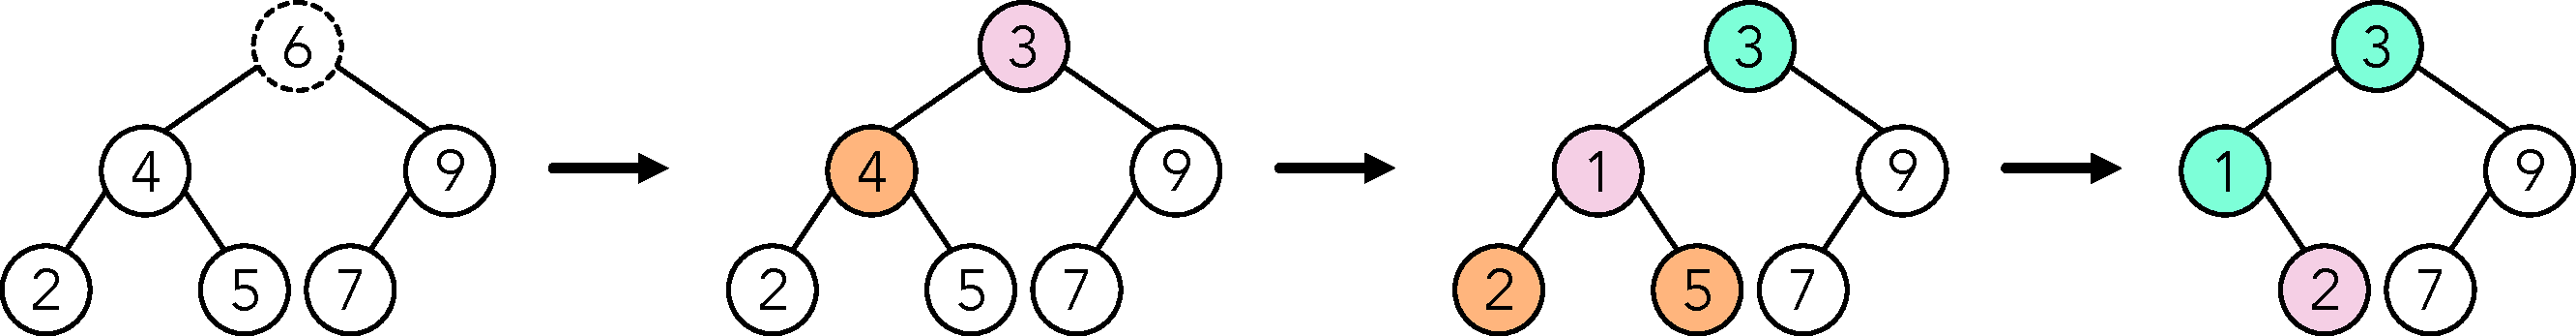
\includegraphics[width=.6\textwidth]{assets/mutate-diagram.pdf}
  \vspace{-2mm}
  \caption{Validity-preserving mutation of a binary search tree, maintaining the
  BST invariant. Mutating the root node from 6 to 3 invalidates the
  4 in the left-hand subtree; the generator 4 with a new random label,
1, then throws away its left subtree (because 1 is the
minimum element of the label range) and relabels 5 to 2.}\label{fig:mutation}
\end{figure}

\medskip

{\em Example-Based Tuning.} Earlier we pointed out that good generators
produce ``realistic'' inputs; one way to ensure this is to tune the generator so
it produces values that are similar to some user-supplied values deemed
realistic. Existing tools make good use of this example-based approach to
tuning~\cite{soremekun2020inputs}, but they do not work with generators as
powerful as monadic generators. We implement a similar algorithm using
reflective generators: we can (1) again, reflect on the choices that lead to a
set of realistic values, and (2) run the generator with {\em new choice weights}
informed by the choices that we saw.

Both of these applications have the potential to significantly improve
testing effectiveness---example-based tuning helps users generate more
realistic inputs, while validity-preserving mutation enables more
automated approaches to improving generator distributions---and we get
{\em both} by upgrading our generators to reflective ones. We
will see additional use cases for reflective generators in the
following sections, and discuss tools that leverage them later in the proposal.

\smallskip

{\bf Status.} We began thinking about reflective generators during a
current NSF project (described in \sectionref{sec:prior}), built a
prototype implementation, and drafted a preliminary progress report
laying out their basic theory~\cite{Frohlich2022}. Some details of
both theory and pragmatics remain to be ironed out; in particular,
while our exploratory performance measurements look promising, a
thorough empirical evaluation forms part of the work during the first
year of the proposed project.

% \amh{Is there a way to make this status report make the success of
% this project sound more assured (if we think it is)? Some of the
% later projects in the proposal depend at least in part on this
% working.}\bcp{Tried tweaking the wording a bit.  I think it's OK.}

\SUBSECTION{Reflective Shrinkers}{sec:shrinking}{2}{2}{Benjamin}
%
Reflective generators' ability to run backward means that they can be used as
a tool for analyzing and manipulating the structure of
generated
inputs.  For example, we can use them to
implement validity-preserving {\em
shrinking} of values to find smaller counterexamples and speed up debugging
without no effort from the user. On its face, this feels similar to
validity-preserving mutation: Can we reflect on choices, shrink these
choices, and
then re-run the generator with the smaller choices? Likely yes! But there are
complications.

Shrinkers need to be more careful than mutators to keep shrunk values faithful
to the original. When mutating, it is generally fine if the mutated value is
occasionally quite different from the original, since the mutator is
trying many values and any that catch a bug are equally good. But a rogue
shrinker runs the risk of confusing the developer. For example, if a
reflective shrinker accidentally creates a visually larger
value---for example, because the relationship between choice sequence length and
output value size is not monotonic---then shrinking might actually make it more
difficult to understand a failing test case. Additionally, if a
reflective shrinker's shrunk choices
produce values that are very different from the original, they may all
avoid triggering the bug, misleading the shrinking algorithm into thinking that
the original value is already as shrunk as possible and causing it to
report a confusing counterexample.

To establish reflective shrinkers as a solution to
validity preserving-shrinking, several important
properties need to be established: for some class of reflective
generators, the associated reflective shrinkers (1) never produce larger values
with fewer choices and (2) always produce shrunk values that are ``close'' to
the original. Formalizing sub-classes of well-behaved reflective generators and
notions of ``shrinker closeness'' should also yield
other potential applications of reflective generators and shrinkers.

The shrinking tools that come out of this work will use reflective generators to
automatically shrink inputs in an validity-preserving way. They will be able to
shrink values that they did not generate (e.g., counterexamples that come from
production), and they will give strong guarantees about the subtleties of the
shrinker behavior. We hope that these tools will mean that developers no longer
need to be intimidated by the idea of shrinkers: they will simply work in the
background, simplifying debugging.

\SUBSECTION{Reflective Fuzzers}{sec:fuzzing}{2}{3}{Benjamin}
{\em Fuzzers} like AFL~\cite{afl-readme} are based on principles
similar to the
ones behind PBT: in particular, they use randomization to exercise many
program behaviors. Fuzzers are popular because they are both capable and
inherently easy to use. The developer need only point the fuzzer at an
executable binary and
wait. But, without help, fuzzers are not very good at finding
bugs when properties have complex preconditions.
Our ultimate goal is a unification of PBT and fuzzing tooling that combines the
powerful automation potential of reflective generators with the usability of
fuzzers.

There are a few existing projects that try to get the best of both worlds by
combining PBT and fuzzing.
For example, the FuzzChick library in Coq~\cite{OLDlampropoulos19fuzzchick}
uses code coverage as guidance for PBT, and the HypoFuzz library uses a
similar approach in Python~\cite{hatfield-dodds_hypofuzz_nodate}. These projects
are demonstrably powerful, but neither benefits from the years of expertise
poured into industrial-strength fuzzers; Crowbar, on the other hand,
does~\cite{dolan2017testing}. Crowbar uses
AFL~\cite{afl-readme}, one of the best-established
fuzzers, to generate random bit-strings that are later parsed into program
inputs. Crowbar does require more user effort than standard fuzzing techniques,
but the coverage guidance means that careful tuning is often not required to get
good testing performance.

We admire Crowbar, but think the idea can be pushed further by building
a variant of Crowbar on reflective generators.
We will start with a classic fuzzing setup, which tries to make the
system under test
crash by passing it a variety of semi-random inputs. Normally, the fuzzer is
``working against'' the parser, in the sense that the parser's job is to reject
invalid inputs and the fuzzer's job is to get past it.  Crowbar's
generators avoid this adversarial relationship because they are
monadic, and can satisfy parer constraints
parser by construction; ours will also be monadic, but also {\em reflective}.

Why a reflective generator? First, we should clarify why any kind of monadic
generator is preferable to grammar-based alternatives. Monadic generators can
straightforwardly generate context-free structures, so they can generate data
satisfying a strictly larger set of constraints than grammar-based ones.
But the beauty of a monadic
generator is that it can be made far more powerful, incrementally, as the
developer's testing needs change. They can start off thinking that they
need only consider the structure of their inputs, but later add more
semantic guarantees (using the extra flexibility of the monadic
presentation) if they find that their generator is wasting too much time
producing invalid values.

A compelling benefit of reflective generators in this scenario is that
their backward interpretation can be used to help seed the fuzzer.
Modern fuzzers often
ask the user for a number of {\em seeds}, input examples that the fuzzer can start from,
to ensure that the fuzzer does not spend ages exploring
inputs that have no hope of exercising the interesting parts of the
system under test. Normally these seeds are easy enough
for the user to write down, since they are simply program inputs, but if
we instead ask the fuzzer to generate sequences of {\em choices}, then
it becomes much more
error-prone (and tedious) to produce seeds by hand.  This is one great use for a
backward interpretation. The user can write down their seeds---either as values
in the program, or as text that can be parsed by the program's parser---and then
the reflective generator can reflect on the choices that produce those seeds.

The reflective generator also provides validity-preserving mutation. Guided by
heuristics, the system can opt to supplement the fuzzer's mutation schedule with
mutations that are obtained by the reflective generator's validity-preserving
mutation (which is more targeted than the mutators provided by the fuzzer). We
expect this to have a significant impact on performance, especially in contexts
where preconditions are relatively sparse and therefore hard for AFL to mutate
correctly.


% \SUBSECTION{Benchmarking}{sec:benchmarking}{1}{3}{Andrew}
% \iflater\todo{Make sure this feels different from Leo's CAREER}\fi
% \bcp{Maybe we should just cut it!}
% %
% The many papers in the PBT literature demonstrate effectiveness with case
% studies, showing that certain bugs in certain systems are caught more quickly
% with one too over another. For theoretical advances, this is often sufficient
% to demonstrate that the paper is worth publishing, but this kind of evaluation
% can be hard to interpret from the perspective of a would-be user. With all of
% the new approaches to generation that we are proposing in this document, and
% considering our goals around usability, we want to do better.

% We will to develop and popularize a robust empirical evaluation framework for
% generators and other PBT techniques. Our first contribution will be an
% infrastructure for easily and extensibly running experiments.  By ``easily,'' we
% mean that we will take on the burden of collecting data and analyzing the
% results, exposing to the user library functions for their particular
% instantiations as needed. We will evaluate a given tool based on (1) the degree
% to which it is able to achieve high code coverage quickly, and (2) the speed
% with which it finds bugs that have been pre-seeded in example programs. By
% ``extensibly,'' we mean that in addition to the two languages (Haskell and
% OCaml/Coq), multiple frameworks (QuickCheck, SmallCheck, QuickChick, etc.), and
% numerous workloads that we plan to support on release, we will design the
% infrastructure so that users can easily add new things along each dimension.

% Our second contribution will codify a library of case-studies and examples as
% {\em benchmarks for PBT}. Similar suites of benchmarks already exist in the
% fuzzing literature~\cite{hazimeh_magma_2021}, but those benchmarks are not
% organized around the particular challenges that PBT tools face. In particular,
% few of the benchmarks deal with the kinds of complex preconditions that PBT
% tools are built to handle. We want to establish a set of challenging tasks that
% can serve as a north star for future improvements to PBT generators and
% bug-finding strategies (including our own!).

% Designs for this project are currently being discussed with Leonidas
% Lampropoulos and his group at the University of Maryland. PI Pierce has a long
% history of successful projects with Prof.
% Lampropoulos~\cite[etc.]{LuckPOPL,goldstein2021dojudgeatest,lampropoulos_coverage_2019,Lampropoulos&18,OLDlampropoulos19fuzzchick}.
% \iflater
% \hg{Is this everything? Probably not...}
% \fi

\SECTION{Validation}{Understanding Testing Effectiveness%
 \pagebudget{3}}{sec:val}

A final set of challenges in maximizing PBT's usability lies in
helping developers
\evaltheme{validate} that their testing is effective. In this section, we
describe a sequence of research efforts to design and evaluate usable developer
tooling for PBT. These projects will contribute new paradigms for tools that
help developers assess whether their generators are generating sufficient and
appropriate inputs (\sectionref{sec:evaluating_distributions}) and whether those
inputs sufficiently exercise their code (\sectionref{sec:tuning}), migrate
counterexamples found by property-based tests into conventional regression tests (\sectionref{sec:counter}),
and understand testing-provoked failures involving complex inputs
(\sectionref{sec:failures}). These projects will be pursued using HCI
methodology, integrating these tools into contemporary interactive development
environments. The success of tools will be evaluated in usability studies
comparing developers' effectiveness and efficiency in writing tests for their
software, and debugging problems discovered by their test suites.  PI Head will
guide tool development efforts, leveraging his
experience designing, developing, evaluating, and deploying novel programming
environments and
tools~\cite{ref:head2015tutorons,ref:suzuki2017tracediff,ref:head2017writing,ref:head2018when,ref:head2018interactive,ref:head2019managing,ref:head2020composing}.

\SUBSECTION{Evaluating Data Distributions}{sec:evaluating_distributions}{2}{3}{Andrew}
%
In comparison to testing techniques like unit testing, PBT draws many
tests from some
random {\em distribution} over possible inputs, rather than writing down a few
concrete individual inputs. The success  of
PBT thus depends on the quality of this distribution---whether
most of its probability mass is on tests that are sufficiently
realistic and diverse. We plan
to develop tooling for
understanding distributions of input data and easily tuning them.

We draw inspiration from related work in HCI that has sought to better expose
the shape of input data distributions including
machine learning datasets
(e.g.,~\cite{ref:hohman2019gamut} and
~\cite{ref:hohman2020understanding}) and sequences of program values
(e.g.,~\cite{ref:kang2017omnicode}).
PBT poses a unique challenge because values produced by generators are
programmatically generated and
can be of unbounded structural
complexity (e.g., lists, trees, and other algebraic data types,
sequences of API calls, ...).
Consider an
example from a participant in our formative study, who wanted to generate
realistic logs of input data, where each log entry included at least a timestamp
and an event type.\proposecut{Such values are not trivially plotted in conventional
visualizations, and it would be prohibitive to review individual examples if the
logs are sufficiently long.} Ideally, a developer would be able to answer
questions like: Are the generated log inputs long enough? Are the even sequences
realistic? This setting requires new kinds of views of data, and tight
developer support for easily defining meaningful views of the data.

\begin{wrapfigure}{r}{0.58\textwidth}
  \centering
  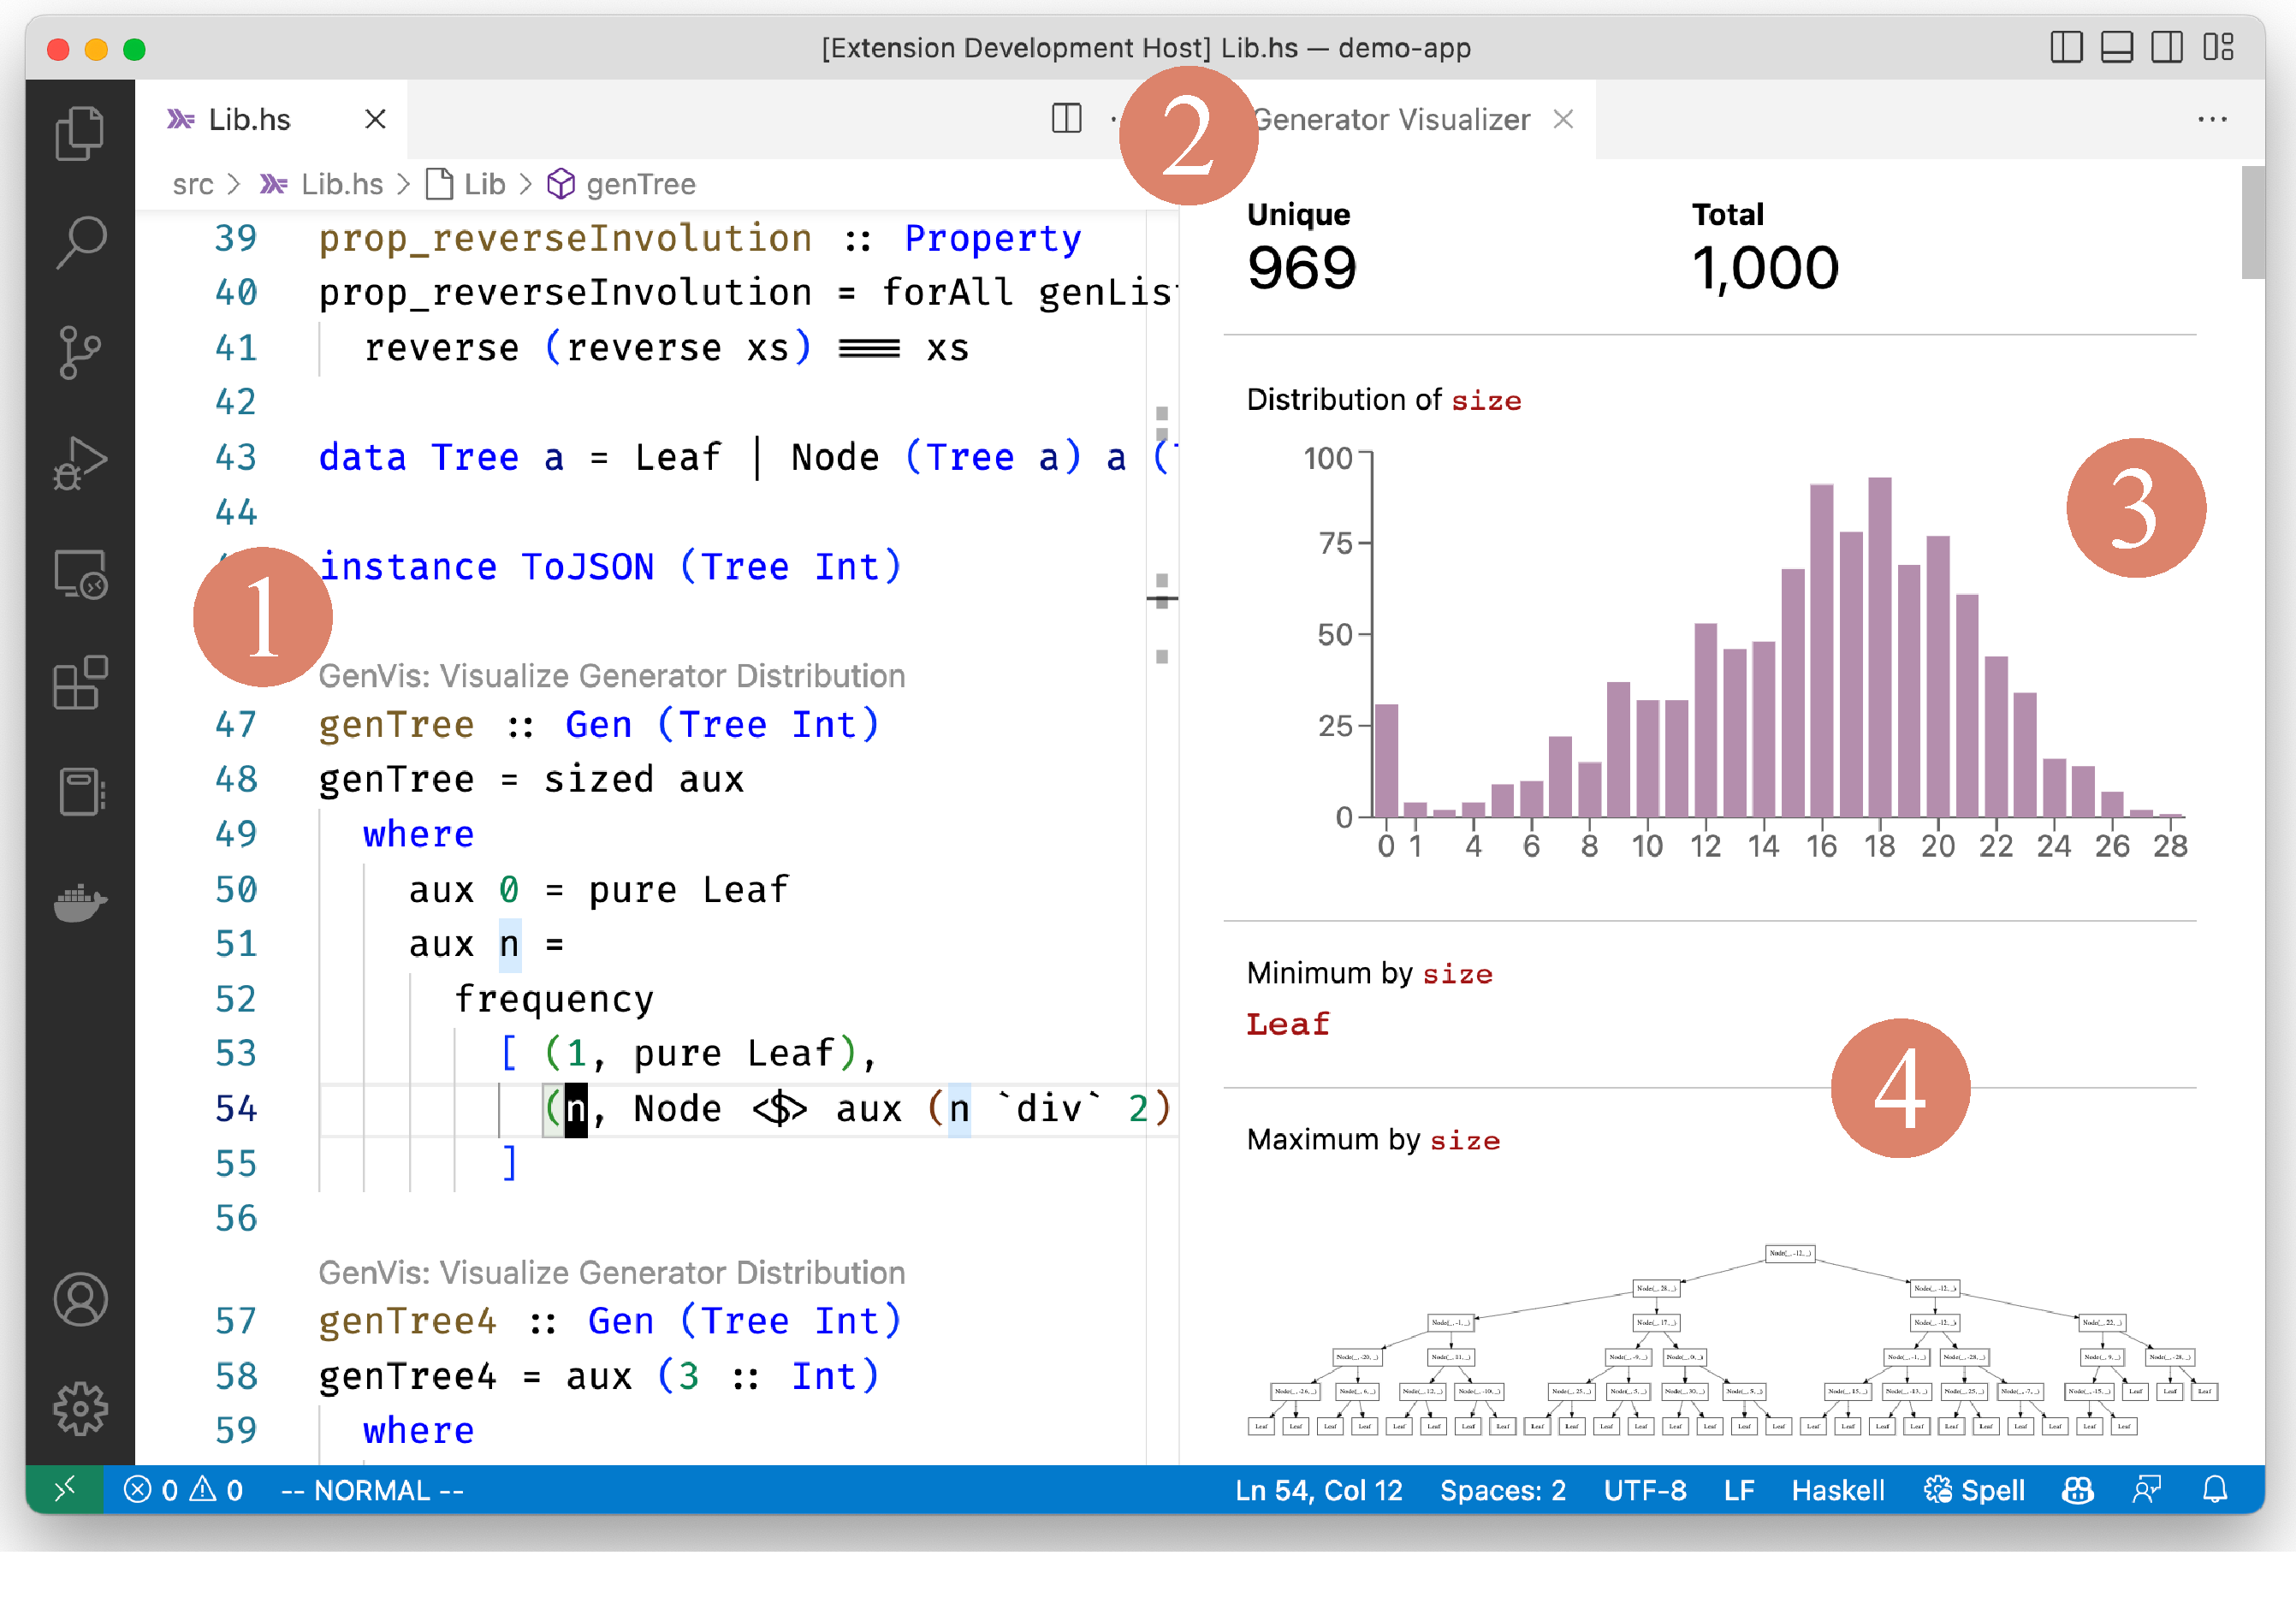
\includegraphics[width=0.58\textwidth]{assets/gen-vis.pdf}
  \caption{An envisioned tool for evaluating data distributions.}\label{fig:gen-vis}
\end{wrapfigure}

We will design new interactive tools that provide rapid,
informative views of input data distributions. The tools will address the
challenges of visualizing generator distributions using a novel combination of
tailored, tried-and-true features for interactive programming environments.

First, our tools will support live, realtime displays of generated values.
Our first goal is to provide
instant, live~\cite{ref:tanimoto1990viva} feedback on the generators. Building
on the tradition of other live functional programming environments
(e.g.,~\cite{tool:lighttable,ref:omar2019live}),
% our environment will provide
% live feedback summarizing many inputs produced by a generator, rather
% than a single one; As testing proceeds,
our environment will sample inputs
output by the generator and
pipe them into data displays (Figure~\ref{fig:gen-vis}), which
will first and foremost show aggregate data views, including aggregate
statistics (Figure~\ref{fig:gen-vis}.2) and visualizations of the distribution
of key features of the data (Figure~\ref{fig:gen-vis}.3). Visualizations will be
generated according to simple recommendation rules, similarly to other recent
exploratory data visualization tools from
HCI~\cite{ref:lee2021lux,wongsuphasawat_voyager_2016,
wongsuphasawat_voyager_2017}. Unique to our project, features to visualize will
be based on awareness of common features of algebraic data types, and extensible
through lightweight user-written code. For example, consider the
\lstinline{log} type
described above. A developer might be interested in the log's
\lstinline{length}, field accessors like \lstinline{event_type}, \lstinline{id},
and \lstinline{timestamp}, filters like \lstinline{is_empty}, and even
aggregators like \lstinline{max_by}. These kinds of features can be
generated automatically for common data types.
% Then the tool will then use
% lightweight type-based program synthesis to compose and combine these functions
% to get features. It may choose to show the \lstinline{length} of a log, but also
% the \lstinline{max_by (fun l -> length l.payload)} (the maximum payload length),
% and even pairs of features like these (which could be viewed as a two
% dimensional feature).

Second, the data displays will be easily extensible, via lightweight customization hooks. If
there are features that the user notices should be extracted, but that the
system cannot come up with itself (e.g., \lstinline{ids_unique}) the user can
write it themselves in companion code alongside their property specifications;
the interface will automatically load those features into the display.

Third, the interface will make it possible to drill down into
individual inputs from a list of samples that can be
filtered by selecting marked visualizations (e.g., choose a bar
of length ``10'' to preview individual inputs with that length). One
challenge will be to provide suitable representations of complex inputs that
will be easy to understand. Some general solutions might be to
pretty-print inputs, provide interactive object browsers like those available
in JetBrains~\cite{tool:jetbrains}, and/or allow a developer to explore an
object using a built-in REPL. Additionally, we will produce DOT
graph~\cite{ellson_graphviz_2002} representations of common kinds of inputs
(i.e., lists, trees) that will provide an at-a-glance understanding of
larger inputs (Figure~\ref{fig:gen-vis}.4).

Finally, our tools will provide live feedback on the input
distribution in the form of in-situ coverage feedback. Like other HCI
prototypes that have shown which lines of code are currently
executing in a running program~\cite{ref:brandt2010rehearse,
  ref:oney2009firecrystal, ref:burg2013record}, ours will be
able colorize code in the editor on the basis of
how frequently each line has been executed while running tests.

The result of these experiments will be the first live tool for generator
feedback and analysis; in the next section, we take it one step
farther to consider how interactive tools can help a developer not
just understand input data distributions, but more directly change
them.

\SUBSECTION{Tuning Data Distributions}{sec:tuning}{3}{4}{Benjamin}
%
Tuning generator distributions is a challenging task, often requiring
significant trial-and-error---changing generator parameters and hoping
that the input data distribution changes in the right way. Approaches
like the one in \sectionref{sec:fuzzing} can help, but manual tuning
is still needed in many cases.
Developers need higher-level ways to describe the kinds of inputs they.

We will design tools to support the direct tuning of input data distributions
through manipulation of generated inputs and data distribution
visualizations. This work will build on the foundation outlined in
\sectionref{sec:evaluating_distributions}. Inspired by recent tools in
the PL+HCI literature
for bidirectional manipulation of programs and their
outputs~\cite{ref:hempel2019sketch, ref:kery2020mage,
  ref:omar2012active, ref:omar2021filling},
we explore reflective generators' potential to support tuning.

The first, general-purpose method for tuning input data distributions will be to
define filters on input data by manipulating aggregate data displays.
For instance, developers will be able to select a range of values from a bar
chart showing input data features and then request that all values generated
within that range are discarded before testing. This approach is flexible,
though it is notably coarse-grained;
it does not influence the implementation of the underlying generator, and
therefore can only go so far in influencing the kinds of values that are
generated.

A second idea is to leverage
reflective generators (\sectionref{sec:reflective}) to change the underlying
generator parameters. Developers will be able to interact with a visualization,
and then the the reflective generator will map those interactions
back to choices
in the generator (e.g., what value to place in a node, or the number of nodes to
produce, etc.), which can then be made more or less frequently. We envision
building tools that show the generator code
side-by-side with visualizations, and where parameter choices in the generator
can update live as the data distribution is manipulated in the visualizations.
Furthermore, developers will be able to interact with individual data points,
expressing that they would like to see more inputs like one that has already
been generated, or that they would like an input similar to a generated input,
but different in a way that they have demonstrated. Together, this tool and the
tool for visualizing generated data distributions will have a synergistic effect
in improving developers' ability to understand and ultimately achieve more
realistic, comprehensive data distributions for their testing.

\SUBSECTION{Counterexamples as Regression Tests}{sec:counter}{2}{2}{Andrew}
%
% After testing has revealed a counterexample to one of their properties
% with their tests, the developer may wish to turn that failure into a
% regression test, to ensure that later
% changes to the code will not reintroduce the same failure.
One pain
point experienced
by informants in our interview study was that it requires considerable work to
transform a failure that was detected by their PBT tools into a
regression test, despite the fact that much of the work involved in doing so
felt mechanical.

We plan to develop usable tooling for transforming failed PBT tests into single
regression tests. What is important to note about this project is that creation
of regression tests is \emph{mostly}, but not entirely, mechanical. In reality,
the creation of regression tests will likely require judicious incorporation of
the developer's input at key decision points. This is particularly the case for
specifying acceptance criteria. For instance, consider a property that checks
that a list insertion function never produces an empty list. In the event of a
failure, a developer may want to produce a regression test checking the
exactness of the result on the failed input (e.g., checking that the insertion
produced a particular concrete list) rather than simply checking that the output
list is non-empty.  Writing a regression test may involve multiple such
choices, including whether to test for exact output, whether to test
intermediate results, and how to initialize inputs.

We will develop an interactive tool that assists developers in creating
regression tests from failed tests. The idea is to first develop
technology for generating sufficiently readable code for regression tests (using
approaches such as Daka et al.'s~\cite{ref:daka2015modeling}), and then provide
in-situ editing assistance along the lines of contemporary interactive
refactoring tools from the HCI
literature~\cite{ref:head2018interactive,ref:barik2016quick,ref:murphyhill2008refactoring,ref:lee2013draganddrop}.
For this unique task of transforming properties into regression tests,
our tool will provide the key features of keeping track of the failed input,
generating starter test code, substituting in correct expected values of the
output by executing corrected code, and supporting developers in rapidly
performing likely edits to regression tests by providing suggestions of
alterations to their code like the ability to generate general property checks
with precise equality checks\bcp{??}. We also hope the results of this work
can inform the
design of other approaches to counterexample extraction, including one that is
proposed for the Hypothesis library in Python~\cite{maciver2019hypothesis}.

% \ifdraft
% \SUBSECTION{Increasing Assurance with More Tests}{sec:more}{3}{4}{Andrew}

% The informants in our interview study admitted to heuristic
% approaches to determining how many tests to run. Many set
% rigid cutoffs such as one-thousand tests, or one minute's
% worth of tests. One reason for these heuristics was that
% developers did not want to lock up their computer's
% computational resources, or delay their other development
% tasks, by waiting for their property-based tests to
% complete. As one of our informants pointed out, this could
% lead to circumstances where bugs were not discovered until
% property-based tests were checked into the continuous
% integration system, when tests were finally conducted at a
% sufficient volume to generate failing inputs \amh{@HG can
% you fact check my paraphrase of this informant's input?}\hg{Technically this was
% a pilot study informant, but I think it's OK}.
% Unfortunately, when failures are detected in continuous
% integration, developers no longer have the context to
% address those problems easily, because they have likely
% moved on to other tasks.

% We believe that, if appropriately designed, a developer's
% PBT tools can help developers get the best of both
% world: they can both increase assurance that their software
% is correct by running more property-based tests, while not
% locking up their computer's resources. We propose to extend
% in-editor testing tools to permit options where developers
% can configure their PBT test drivers to continue testing
% software in the background by default, without requiring a
% developer's explicit input. These tools will scan a
% developer's environment for property-based tests, divide
% time proportionally between the various tests, and capture
% the results in a digested form. To reduce the likelihood of
% breaking a developer's focus, errors will be marked through
% subtle annotations in the code (e.g., icons in the line
% margins) when one has been detected. Developers can also
% request alerts that can report failures instantaneously,
% should they wish to address any discovered failures right
% away.

% \hg{This section needs honing; right now it's just what I wrote in my thesis
% proposal, and it's too high-level} \amh{Is this a user
% interface project devoted to figuring out ways of invoking
% and keeping tabs on long-running tests during solo
% programming? Or is it a project around proposing better
% software engineering process that gives the right amount of
% time to long-running PBT tests?}
% \hg{Good question. I kind of naively hoped it was a UI project that both helped
% users invoke and keep tabs of tests in the background AND pushed them towards
% software engineering processes that gave PBTs appropriate space to operate. But
% now that I think about it that seems like a lot at once. Honestly I think the
% cultural shift in SE (potentially backed by some large-scale software tools) is
% the more impactful angle, but I don't know if we can argue that we know how to /
% want to do that}
% \bcp{Delete the section?}
% \amh{I tried this section again, trying to spell out in more
% detail my updated conception about what would be useful and
% magical about this tool. Can someone else take a look at it
% and make the decision of whether to remove the section?}
% \hg{I think it's better, but it's still pretty vague and flat. I wish there was
% a specific example of an interaction that I could say ``oh yeah, why don't I
% have that?'' As written, it sort of feels like the devil is in the details and
% we didn't actually give an details}

% % It is likely that PBT tools could play a role in improving this state of
% % affairs. For example, one could take inspiration from some theorem
% % provers~\cite{berghofer2004random} and create a system in which properties are
% % checked locally but in the background, as the programmer works on other things.
% % This avoids waiting time while potentially being less frustrating than running
% % in CI, since bugs would likely be found while the programmer still had the code
% % ``paged in.'' Alternatively, one might design a PBT system with CI in mind,
% % providing automated features for deferring property failure notifications until
% % a specified time or turning failing properties into unit tests that can be saved
% % for future testing.

% \fi

\SUBSECTION{Interactive Shrinking and Debugging}{sec:failures}{3}{4}{Andrew}
%
One of the challenges in using PBT is understanding why
a given counterexample triggers a bug.  We will design interactive
tools to help in this process.

First, we will design tools that build on
shrinkers~\cite{hughes_quickcheck_2007,arts_shrinking_2014} to help developers
understand counterexamples. Automatic shrinking, even when done via reflective
shrinkers as we discuss in \sectionref{sec:shrinking}, can be opaque, and
shrinkers often make suboptimal decisions that an individual developer might be
able to make better.
Drawing inspiration from approaches in recent HCI literature that support
interactive code reduction through iterative, incremental
experimentation~\cite{ref:lim2018ply,ref:head2018interactive,ref:holmes2012systematizing,ref:hibschman2016telescope},
we will design aids for rapid, incremental, interactive shrinking of complex
inputs into simpler inputs. The key feature we will develop is the ability to
shrink inputs semi-automatically by pruning the input's contents and structure in an interactive
object viewer, similar to the kinds of object viewers available in contemporary
debuggers like in the JetBrains IDE~\cite{tool:jetbrains}.
The interactive shrinker will display the \emph{valid} ways
in which an input can be pruned, but the choice of exactly what to prune will be
up to the human. We will rely on reflective generators to provide the insights
into which parts of the structure correspond to choices that can be pruned, and
these pruning points will be made
visible in the object viewer. As a developer prunes the input, they will receive
continuous feedback as to whether it still causes a test to fail or not.
Developers will ultimately be able to
reduce complex counterexamples into simpler ones that are
easier to reason about when looking for bugs.

% Developers will also be alerted if the execution path
% through the code has changed as a result of shrinking the input. In some
% circumstances, this will indicate an undesirable change in the shrunken input,
% and in other cases, such changes in execution paths may be permissible (e.g., if
% the change in the input has led to a reduction in the number of cycles through a
% loop).

% \amh{Could we indicate on top of an object explorer which
% parts of the structure, if changed, would end up leading to
% a different test result, or preserving it?}
% \hg{To a point... You'd run into exponential blowup pretty much immediately, but
% depending on the scale of the input it could be doable}

% Other related projects:
% Whyline~\cite{ref:ko2009finding}.

In addition to developing novel interaction techniques for simplifying inputs,
we will also develop systems for helping developers locate code that, if
changed, would resolve the failure. Rather than explicitly encoding
relationships between generated outputs and their dependencies on
code~\cite{ref:ko2009finding}, we will instead help the developer
understand where the execution paths of a given counterexample diverges from
successful yet very similar inputs. Leveraging the parametric nature of the
reflective generators, we will generate inputs in a space ``around'' a
counterexample and identify which ones no longer cause a failure.  Then, we will
execute the program up to the point where the traces of the programs begin to
diverge, and we will drop the programmer into a debugging environment where
they can query the state of the program and step through the remainder of the
execution. PI Head has prior work designing debugging tools that help
programmers understand trace divergences in an educational
settings~\cite{ref:suzuki2017tracediff}; the work of this project would be to
bring this technology into professional programming environments where traces
for similar inputs are abundant.

\SECTION{Education}{Advancing PBT in the Broader Culture\pagebudget{1}}{sec:ed}
%
Our goal is to make PBT not only usable but {\em
used} in settings where it offers benefit; such a goal requires advances in PBT
\edutheme{education} for
new and experienced programmers alike. In this section, we describe
our plans to develop
course materials for instructors who want to integrate PBT into
undergraduate data structures courses (\sectionref{sec:1210}),
%
tooling to help students write their first properties
(\sectionref{sec:interactive}),
%
and course materials for instructors to integrate PBT into
early-stage computer science curriculum (\sectionref{sec:1210}).


\SUBSECTION{``When to Specify It!''}{sec:whento}{1}{2}{Benjamin}
%
Our first pilot study with users of PBT suggested that developers struggle to
come up with specifications that are worth
testing~\cite{goldstein_problems_2022},
but
our follow-up interviews at Jane Street suggest that the developers there
rarely have the same problem. It seems that the Jane Street developers had
a tacit
understanding of ``no-brainer'' situations where PBT was an obvious
choice---situations where properties were easy to find and where PBT provided
much more thorough testing than other common techniques---and they limited their
use of PBT to these situations.
While experienced PBT users do also apply it in
high-cost / high-benefit situations, we believe
focusing on easier cases is the best way to drive adoption.

We aim to produce authoritative resources that help developers understand
high-leverage situations for PBT. We will begin with an effort
tailored to the academic community: a survey paper with the
aspirational title ``When to Specify It!'' in homage to John Hughes'
widely-viewed tutorial ``How to Specify It!''. This survey will
document the range of high-leverage scenarios identified in our formative
research, including cases like
\begin{enumerate*}[label=(\arabic{enumi})]
\item ``these two functions (e.g., a parser and a printer) should round-trip,''
\item ``this data structure (e.g. a set, map, etc.) should obey algebraic laws,''
\item ``this stateful module should uphold an invariant,''
\item ``these two programs should behave the same'' (e.g., because one
is an optimized version of the other),
and
\item ``this program should not crash.''
\end{enumerate*}
This list will be further expanded with our follow-up surveys with broader
communities of developers~(\sectionref{sec:survey}), a comprehensive
review of case studies that appear in
the academic literature, and an examination of open source projects across a
variety of different software ecosystems using PBT (e.g.,
QuickCheck/Haskell, Hypothesis/Python, Quickcheck/OCaml).

Building on the strong foundation of the survey, we will distill our findings
into media directly tailored for developers. First, we will write up
approachable developer documentation in partnership with our industry
collaborators, to be read among the first resources of any developer
documentation on PBT tools. We will work with our industry collaborators to
disseminate this documentation in blogs and incorporate it into tool
manuals. Then, we will present the findings as a talk at a
major professional developer conference.

\SUBSECTION{Interactive Property Specification}{sec:interactive}{3}{4}{Andrew}
%
Even when a developer knows when properties are useful in the abstract,
they may still have trouble writing their first properties
for real projects. We plan to develop prototype interactive tools that help
programmers compose their first properties in an educational setting.

The vision of this work is to provide a mixed-initiative~\cite{ref:allen1999mixed}
tool, where a student and their code editor work together to arrive at a
meaningful property. Extending prior work on property extraction techniques (see for
instance~\cite{ref:ammons2002mining, ref:le2018deep, ref:claessen2010quickspec,
smith_discovering_2017}), the idea is to help students compose properties that
are not just accurate descriptors of the system, but significant in reflecting
important program behavior. We will build an interface on top of a property
extractor which allows students to write their first properties which supports a
student by allowing them to (1) identify areas of code likely to lead to adverse behavior;
(2) providing unit test cases that represent special cases of more general
properties; and (3) selecting attributes of data types in the source code, or
of input and output data in a debugging REPL, relevant to the property. These
features will allow a student to more rapidly map from behaviors they can
observe or specify in familiar ways, and see how those behaviors are cast into
the language of their property checker.
%
The tool will be designed for use in Penn's upper division Haskell
course (CIS 5520) and therefore implemented on top of
Haskell's property
generator tool, QuickSpec~\cite{ref:claessen2010quickspec}.

\SUBSECTION{PBT for Undergraduates}{sec:1210}{1}{4}{Both}
%
Education can act as a force multiplier to make technologies more usable.
When tools or techniques become standards in undergraduate curricula,
students help bootstrap adoption of those tools and techniques in industry. We will
integrate PBT into some of the earliest coursework that undergraduate students
take, targeting introductory level data structures
curriculum. As noted in \sectionref{sec:whento}, testing well-defined data
abstractions is one of the high-leverage scenarios for using PBT, making data
structures a powerful anchor for demonstrating the power of PBT. Building on the
foundation of recent PBT instruction in data structures
courses~\cite{wrenn2021using,nelson2021automated}, we will integrate PBT into
Penn's CIS 1210 course on data structures. We
will evolve the curriculum to emphasize themes in PBT that have arisen from our
formative research to help students identify powerful circumstances for
using PBT, including methods for writing great generators, understanding
generators, considering properties as documentation, and expanding one's
thinking around the scenarios where PBT is suitable
(see~\sectionref{sec:whento}). We will evaluate the impact of these new
instructional approaches on students' ability to leverage PBT in final projects,
disseminating our findings in publications at computer science research venues.
The instructional materials we develop will be made public for instructors at
other institutions to adapt into their own curricula.

\immediate\closeout\workplanfile
\SIMPLESECTION{Plan of Work\pagebudget{.7}}{sec:plan-of-work}

\bcp{I've moved the text that was here to a separate supplemental
  document, but we'll probably want to say something short in the main
  project description (either here or, better, toward the top) about
  synergy and coordination, with a pointer to that document.}

% \begin{figure}[ht]
%   \centering
%   \vspace*{-1in}
%   \hspace*{-.4in}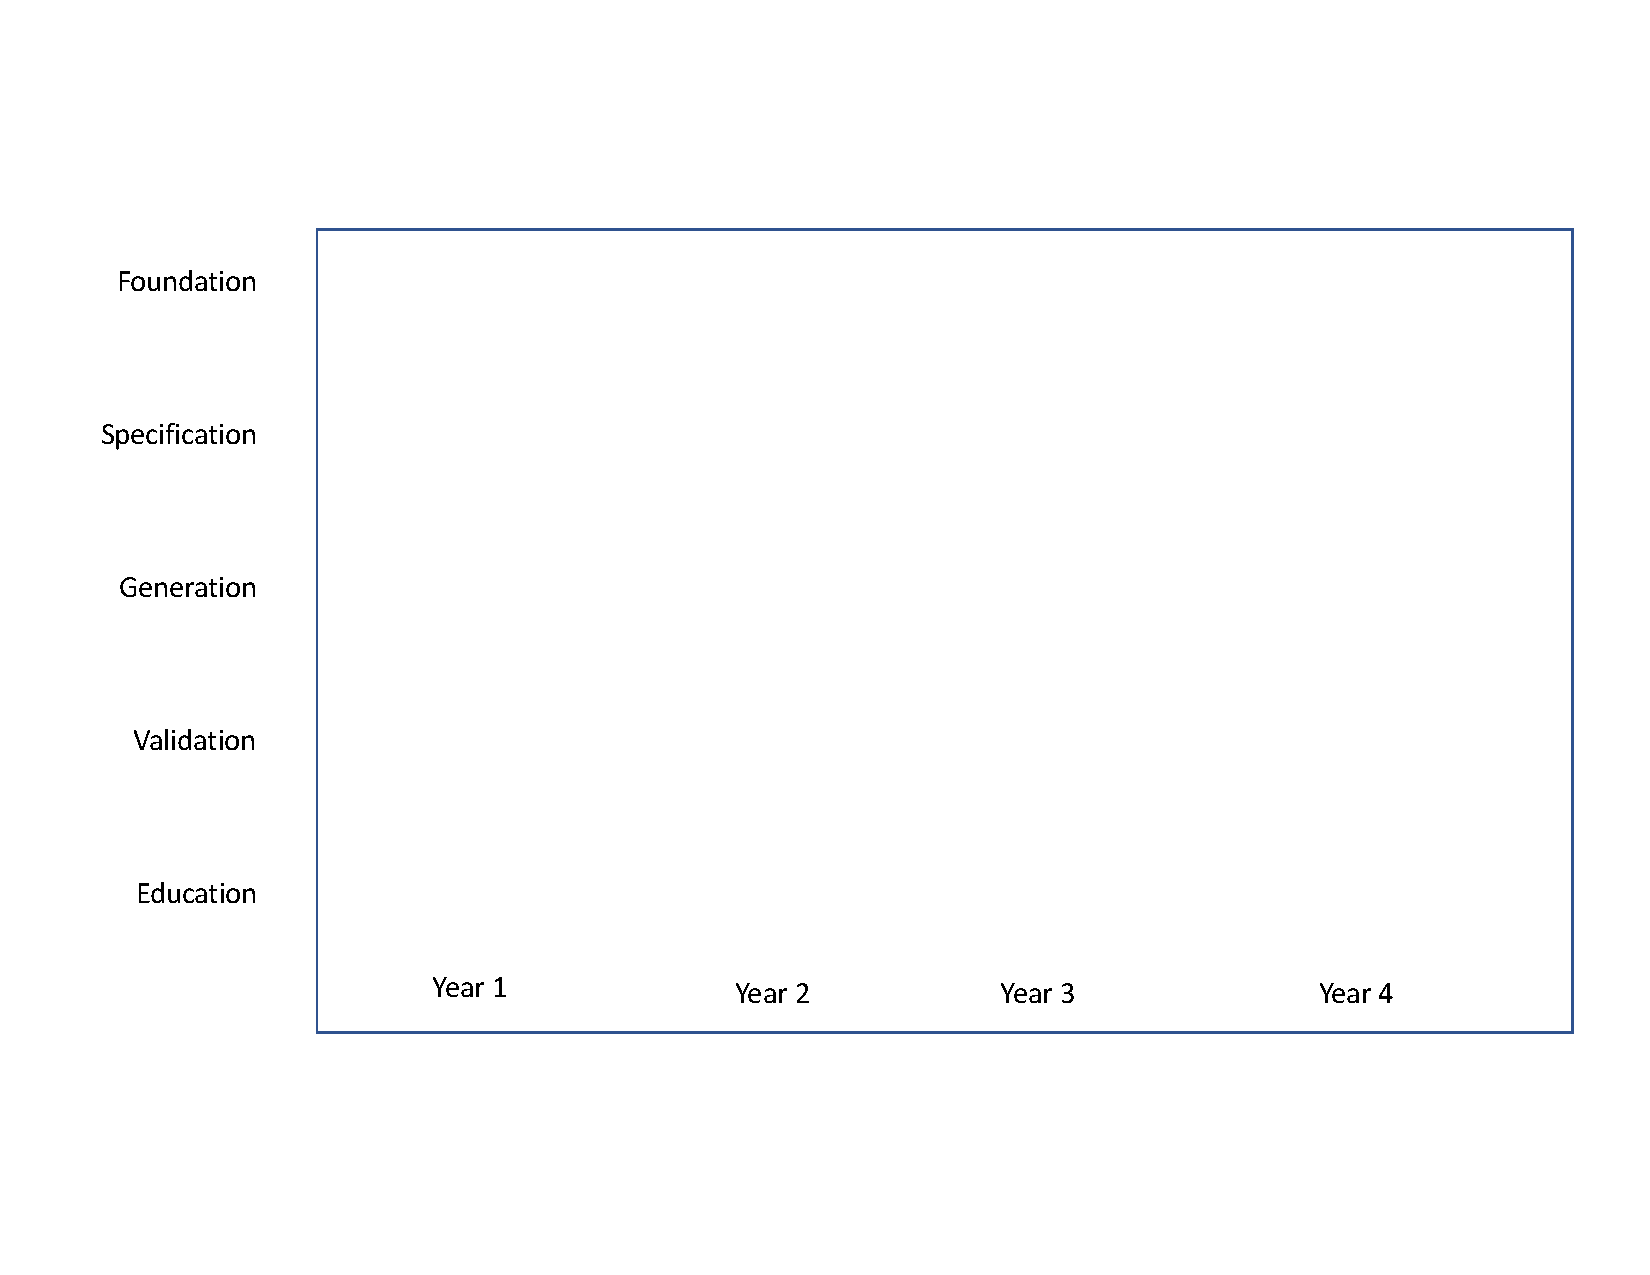
\includegraphics[width=1.1\textwidth]{assets/workplan.pdf}
%   \vspace*{-1.3in}
%   \caption{Plan of work.}\label{fig:workplan}
% \end{figure}

% \vspace*{-.4in}


\SIMPLESECTION{Broader Impacts%
 \pagebudget{.5}}{sec:broader-impacts}

\noindent{\bf Educational Benefits.}
%
The most immediate broad impact of the proposed work will be the
development of educational materials. Educational activities will be
coordinated with the rest of the work, and they are integral to the
project's overall goal of making PBT a standard testing methodology,
readily available to every industrial developer.  Specific pedagogical
threads within the project are described in~\sectionref{sec:ed}.

As an auxiliary goal around education, broadly construed, we will also work to
publicize and communicate the benefits of PBT in the broader computer science
research community. As part of these efforts, we will write an article on PBT
for the Communications of the Association for Computing Machinery (CACM).

\smallskip
\noindent{\bf Mentoring and Diversity.}
%
The majority of requested funding will support formative research
experiences and mentoring for graduate students. We
also plan to work with undergraduate students during this project;
they, too will benefit from the research experience. Each graduate
student will have leadership responsibility for multiple facets of the
project, including co-supervising interested undergraduate
researchers.

The PIs will recruit students for this project with a mind towards making
the research area reflective of diversity in the US, and Pennsylvania specifically.
The PIs have had made inroads broadening participation of women in their
groups (1/3 of Pierce's direct Ph.D. mentees are women, as are 2/3 of PI
Head's). That said, a particular area of focus going forward will be on increasing representation of
other underrepresented groups, including Black and Latinx students. Pierce (along with Penn colleagues Zdancewic and Weirich)
was recently informed that he will likely receive funding for an
NSF REU program that will involve 24 undergraduates (8 per
year for three years), selected specifically with an eye to diversity;
some will certainly work on this project. See the appendix on Broadening Participation in Computing for more
details.

\smallskip
\noindent{\bf Benefits to Society.}
%
The project's goals will also be served by open-source distribution of the tools
built during the project. Key systems will be engineered and documented to a standard
that makes them immediately useful to engineers and students: the projects around
improved generation and shrinking, PBT over logs, and evaluating data
distributions will be particular targets for widespread
dissemination. The remaining projects will be published under a permissive
open source license to serve as models for similar tools for other programming languages and environments.

The project also represents an excellent opportunity for strengthening
collaborations between university researchers and industrial advocates of PBT.  Our
ongoing user study at Jane Street has been carried out with the
enthusiastic support of their developers and management, and we hope
to continue using them as a testbed for prototypes of the tools we
will build.  Similarly, we are in active discussions with the
developers of the Hypothesis testing tool for Python, who are keenly
interested in the results of the studies in
\sectionref{sec:survey}.

Longer term, better testing means better software.  As software
systems have grown to the gigantic scale seen today, good testing
methodologies and tools (unit testing tools, test-first design
methods, etc.) have come to play an ever more crucial role.  Adding a
powerful new testing tool to programmers' arsenals will further boost
this part of the development process, leading to software of every
sort that is more robust, more reliable, and less expensive to build.


% \proposecut{See the Collaboration Plan for
% more.}

% The Project Description must contain, as a separate section within the narrative, a section labeled ``Broader
% Impacts of the Proposed Work". This section should provide a discussion of the broader impacts of the proposed
% activities. Broader impacts may be accomplished through the research itself, through the activities that are
% directly related to specific research projects, or through activities that are supported by, but are complementary to
% the project. NSF values the advancement of scientific knowledge and activities that contribute to the
% achievement of societally relevant outcomes. Such outcomes include, but are not limited to: full
% participation of women, persons with disabilities, and underrepresented minorities in science, technology, engineering, and
% mathematics (STEM); improved STEM education and educator development at any level; increased public
% scientific literacy and public engagement with science and technology; improved well-being of individuals in
% society; development of a diverse,globally competitive STEM workforce; increased partnerships between
% academia, industry, and others; improved national security; increased economic competitiveness of the United
% States; and enhanced infrastructure for research and education.

\SIMPLESECTION{Results from Prior NSF Support\pagebudget{.5}}{sec:prior}

% If any PI or co-PI identified on the project has received NSF funding (including any current
% funding) in the past five years, in formation on the award(s) is required,
% irrespective of whether the support was directly related to the proposal or not.
% In cases where the PI or co-PI has received more than one award (excluding amendments),
% they need only report on the one award most closely related to the proposal. Funding includes not just salary
% support, but any funding awarded by NSF. The following information must be provided:\\

\emph{\underline{PI Pierce}}: (NSF 1955565) ``Collaborative Research:
SHF: Medium: Bringing Python Up to Speed'' (\$437,999,
7/2020--6/2023), with co-PIs Michael Hicks (Maryland) and Emery Berger
(Amherst).
The project aimed to dramatically increase the performance and
correctness of applications written in Python by developing novel
techniques for performance analysis, optimization, run-time systems,
property-based random testing, concolic execution, and program
synthesis. It developed both
novel performance analysis tools and optimizations and novel automatic
testing frameworks. These were largely tailored to and implemented for
Python, but applicable in other, similar languages.
%
{\bf Intellectual Merit.} The project involved work on both
performance measurement (mostly at Amherst and Maryland) and PBT (mostly at Penn
and Maryland).  Specific threads of work involving Penn included
building an early
version~\cite{Frohlich2022} of the Reflective Generators described in
\sectionref{sec:reflective}, carrying out the pilot study of PBT in Python
mentioned in the motivation section
above~\cite{goldstein_problems_2022}, and building on the idea of
freer monads from functional programming to develop ``free
generators,'' which unify parsing and
generation~\cite{goldstein2022parsing}, presented a principled
automatic testing framework for application-layer
protocols~\cite{Li2021:MBToNA}, and developed and released a freely
available mutation testing framework for Python, called {\tt
  pytest-mutagen}~\cite{pytestmutagen}, and applied ideas from
combinatorial testing, a widely studied testing methodology, to modify
the distributions of random test-case generators so as to find bugs
with fewer tests~\cite{DBLP:conf/esop/GoldsteinHLP21}.
%
{\bf Broader Impacts.} Project results and open-source software
products are being used to increase the
performance and correctness of Python applications.
Educational impact has included training both graduate and
undergraduate students, including a female PhD student at Penn, Jessica
Shi.
%
{\bf Publications (involving Penn).} \cite{Frohlich2022,DBLP:conf/esop/GoldsteinHLP21,
  goldstein2022parsing, goldstein_problems_2022, Li2021:MBToNA}.
{\bf Research Products (from Penn).} \cite{pytestmutagen}.

\emph{\underline{PI Head}} has not previously received NSF support.

% \SUBSECTION{Proposed Study}
% The Project Description should provide a clear statement of the work to be undertaken and must include:
% objectives for the period of the proposed work and expected significance; relation to longer-term goals of the PI's
% project; and relation to the present state of knowledge in the field, to work in progress by the PI under other
% support and to work in progress elsewhere.
%
% The Project Description should outline the general plan of work, including the broad design of activities to be
% undertaken, and, where appropriate, provide a clear description of experimental methods and procedures.
% Proposers should address what they want to do, why they want to do it, how they plan to do it, how they will
% know if they succeed, and what benefits could accrue if the project is successful. The project activities may be
% based on previously established and/or innovative methods and approaches, but in either case must be well
% justified. These issues apply to both the technical aspects of the proposal and the way in which the project may
% make broader contributions.

\ifdraft
\section*{Stuff to think about once the document stabilizes}

\todo{GPG: To increase the diversity of the reviewer pool, CISE actively encourages each proposer to include a list of suggested reviewers (including email addresses and organizational affiliations) whom they believe are especially well qualified to review the proposal and are not conflicted with project personnel. Suggestions for reviewers from groups underrepresented in computing are especially encouraged. Proposers should follow the guidance in PAPPG Chapter II.D.1.}

\todo{GPG: Does the plan incorporate a mechanism to assess success?}

\todo{Webinar: Staff support is normal.  Needs to justified not only
  in the body of the proposal but also carefully called out in the
  budget justification.}

\todo{GPG: Issues of fairness, ethics, accountability, and
  transparency (FEAT) are important considerations for many core
  topics in computer and information science and engineering. In
  projects that generate artifacts ranging from analysis methods to
  algorithms to systems, or that perform studies involving human
  subjects, PIs are encouraged to consider the FEAT of the outputs or
  approaches.  (We should touch on this point somewhere.)}

\fi
